\section{Actividades con el repositorio GitHub}

\subsection{Implementación del Ejercicio 1}

\begin{itemize}
	\item Mostrando resultado del ejercicio 1, 
\end{itemize}
\begin{figure}[H]
		\centering
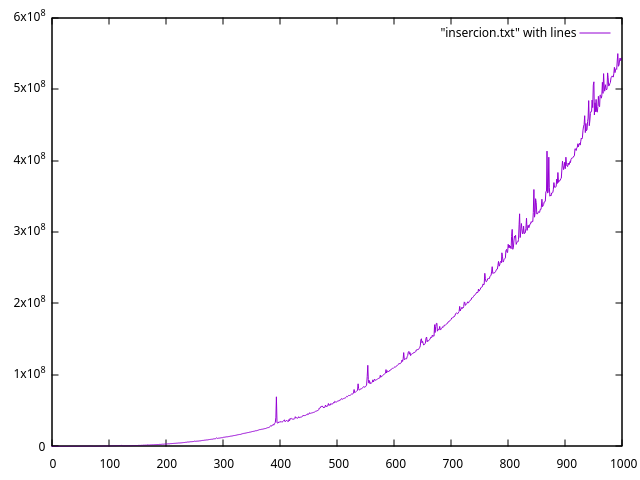
\includegraphics[width=0.8\textwidth,keepaspectratio]{img/capEjercicio1.png}
		%\includesvg{img/automata.svg}
		%\label{img:mot2}
		%\caption{Product backlog.}
	\end{figure}

\subsection{Implementación del Ejercicio 2}
\begin{itemize}
	\item Mostrando resultado del ejercicio 1, 
\end{itemize}
\begin{figure}[H]
		\centering
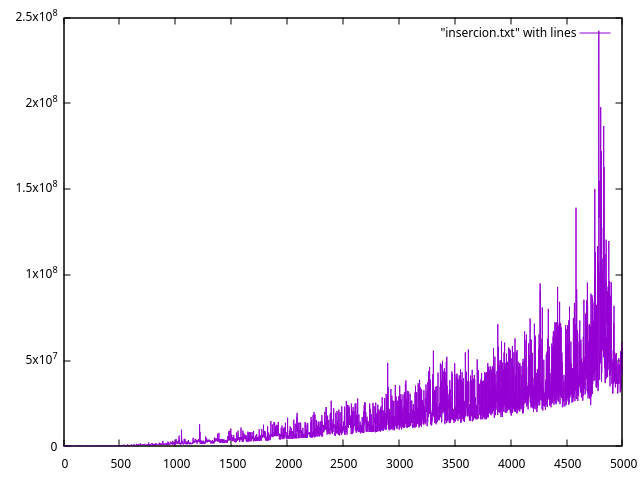
\includegraphics[width=0.8\textwidth,keepaspectratio]{img/graph.png}
		%\includesvg{img/automata.svg}
		%\label{img:mot2}
		%\caption{Product backlog.}
	\end{figure}

\subsection{Commits}
\begin{itemize}
	\item Commit del ejercicio 1.
	\begin{figure}[H]
		\centering
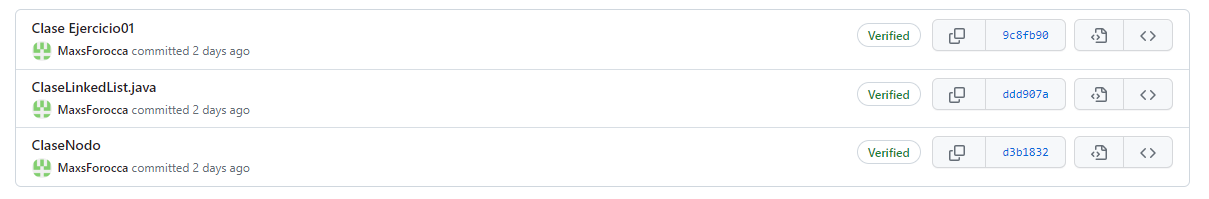
\includegraphics[width=0.8\textwidth,keepaspectratio]{img/commit1.png}
		%\includesvg{img/automata.svg}
		%\label{img:mot2}
		%\caption{Product backlog.}
	\end{figure}
	\item Commit del ejercicio 2.
	\begin{figure}[H]
		\centering
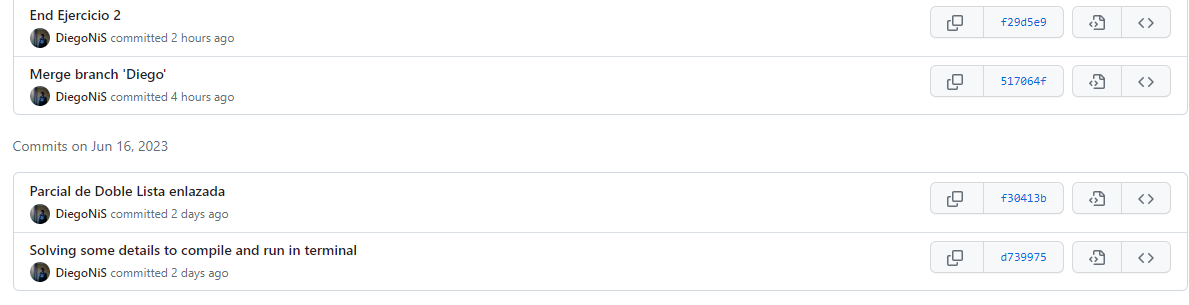
\includegraphics[width=0.8\textwidth,keepaspectratio]{img/commit2.png}
		%\includesvg{img/automata.svg}
		%\label{img:mot2}
		%\caption{Product backlog.}
	\end{figure}
\end{itemize}

\subsection{Estructura de laboratorio 04}

\begin{lstlisting}[style=ascii-tree]
lab04/
|--- Ejercicio1
	|--- Ejercicio1.java
	|--- LinkedList.java
	|--- Nodo.java
|--- Ejercicio2
	|--- DoubleLinkedList.java
	|--- Test.java
	|--- Node.java
	|--- graph.PNG
|--- EjerciciopPrueba
	|--- DoubleLinkedList.java
	|--- insercion.txt
	|--- LinkedList.java
	|--- LinkedListTest.java
	|--- Node.java
	|--- Test.java
|--- latex
    |--- img
        |--- logo_abet.png
        |--- logo_episunsa.png
        |--- logo_unsa.jpg
        |--- CapEjercicio1.png
        |--- Commit1.png
        |--- commit2.png
        |--- graph.png
        |--- net.png
    |--- .gitignore
    |--- Laboratorio-eda-grupo6.pdf    
    |--- Laboratorio-eda-grupo6.tex
    |--- actividades.tex
    |--- cabecera.tex
    |--- caratula.tex
    |--- github.tex
    |--- materiales.tex
    |--- preguntas.tex
    |--- referencia.tex
    |--- rubrica.tex
    |--- tarea.tex
    
|---JavaPlot
|---README
\end{lstlisting}    

  